\chapter{Calculating Temperature Changes using the fMRI BOLD Response}
  \section{\label{sec:tempmodelintro} Introduction}
  Using fMRI to find brain temperature is enticing because it is noninvasive.  Existing efforts to model temperature changes be can categorized into two classes.  The first class approaches the problem by considering a single region of interest (ROI) deep within the brain (single-voxel approach) while the second approach considers the brain and head as an entire system (multi-voxel approach). The single-voxel approach is unable to explain the experimental observation of an increase in temperature during a task; however a multi-voxel approach is able to account for this observation.

  %%  SINGLE VOXEL APROACH %%
    \subsection{\label{sec:singlevox} Single-Voxel Methods}
    Numerous single-voxel approaches have been created ~\citep{sotero2011,yablonskiy,trubel}~which differ largly only in their formulation of Penne's Bioheat Eqution~\citep{pennes}.  Although different approaches consider different contributions to the temperature change, they all narrow the problem down to a single region of interest.  By simplifying the model, the heat equation can be simplified and the calculation is much easier to undertake.  However, since the brain is not homogenous, the values used for parameters such as heat production and thermal conductivity are taken from an average of the tissues.  As a result, this reduces the level of accuracy these models can achieve.
    
    The most recently published iteration of a single-voxel model was published by~\citet{sotero2011} in~\citeyear{sotero2011}. Their formulation of Penne's Bioheat Equation is as follows~\citep{pennes, sotero2011}.
    %%%%%%%  Bio-heat Equation %%%%%%%%%%%%
    \begin{align}
      \label{eq:bioheat}
      C_{tissue} \frac{dT(t)}{dt} &= (\Delta H^{\circ}-\Delta H_{b}) CMRO_{2}\mid_{0} m(t) - \rho_{b} C_{b} CBF\mid_{0} f(t) (T(t) - T_{a}) \nonumber \\
      &\qquad {} - \frac{C_{t}}{\tau} (T(t)-T_{0})
    \end{align}
    where C$_{tissue}$ is the specific heat of the tissue, $\Delta H^{\circ}$ is the enthalpy released in the oxidation of glucose, $\Delta H_b$ is the enthalpy used to release oxygen from hemoglobin, CMRO$_2 \mid_0$ is the metabolic rate of oxygen at rest, $\rho_b$ is the blood density, C$_b$ is the specific heat of blood, CBF$\mid_0$ is the cerebral blood flow at rest, T$_a$ is the arterial blood temperature, C$_T$ is the specific heat for the tissue, and $\tau$ is a time constant for conductive heat loss.  The values used are provided in~\cref{tbl:soteroparams}.
    
    One advantage of using~\cref{eq:bioheat} is that the resting state temperature can be analytically determined by substituting $\frac{dT(t)}{dt} = 0$~\citep{sotero2011}.
    %%%%%%%  Resting state temperature %%%%%
    \begin{equation}
      \label{eq:restingtemperature}
      T_{0} = T_{a} + \frac{(\Delta H \mid^{\circ} - \Delta H_{b}) CMRO_{2}\mid_{0}}{\rho_{B} C_{B} CBF\mid_{0}}
    \end{equation}
    If the values provided in~\cref{tbl:soteroparams} are substitued into~\cref{eq:restingtemperature}, a resting temperature of 37.3057\degree C is found (using T$_a$ = 37\degree C).  Regardless of the arterial blood temperature, since the second term of~\cref{eq:restingtemperature} is always positive the resting state temperature will always be greater than the arterial blood temperature. Thus, an increase in blood flow will remove heat from the ROI, thereby lowering the temperature. As will be further discussed in~\cref{sec:theoreticalresults}, this is an acceptable result for the majority of the brain; however a multi-voxel approach reveals that a region of the brain exists where a single-voxel model is unable to predict temperature changes.  Since it is a simpler model than a multi-voxel model, it is easier to first understand the principles of Penne's Bioheat Equation using this model before discussing how it can be applied to the entire head. 
    
    While~\cref{eq:bioheat} is appears complicated, conceptually Penne's Bioheat Equation can be easily understood:
    \begin{align}    
      \label{eq:soteroexplaiend}
      heat\ capacity\ &*\ change\ in\ temperature\ =\ heat\ generated\ by\ metabolism\nonumber \\ 
      &\quad {} -\ heat\ lost\ due\ to\ convection\ -\ heat\ lost\ due\ to\ conduction\nonumber\\ 
      &\quad {}  -\ heat\ lost\ due\ to\ radiation\
    \end{align}
    The system is a balance between heat generation (metabolism) and heat transfer (conduction, convection and radiation).  The direction of heat transfer by convection is determined by the difference between the voxel temperature and the arterial blood temperature (T$(t) - $T$_a$).  Similarly, the direction of heat transfer by conduction is determined by the difference between the voxel temperature and the temperature of the surrounding tissue (T$(t) - $T$_0$).  Since T$_a$ is less than T$_0$, an increase in blood flow ($f(t)$) will remove heat from the voxel thereby decreasing the temperature.  Conversely, an increase in metabolism ($m(t)$) without a corresponding change in blood flow, will result in tissue warming.  \Cref{eq:bioheat} omits the effect of radiation because the contribution is small compared to the other terms.  As we will see in~\cref{sec:ThermalImaging}, mid-infrared photons are reabsorbed by tissue within \Gtilde 10--100 \textmu m~(\cref{fig:waterabs}) so any energy lost due to radiation does not travel very far compared to the ROI size.
    
    %%  MULTI VOXEL APPROACH  %%
    \subsection{\label{sec:multivox} Multi-Voxel Methods}
    The multi-voxel approach to calculating brain tissue temperature alleviates many of the issues that a single-voxel approach has.  The most prominent advantage a multi-voxel approach has is a result of it accounting for a voxel's location relative to the surface of the head and other voxels.  By accounting for a voxel's location, the same BOLD response in two different locations can have vastly different effects on the local tissue temperature (more on this in~\cref{sec:theoreticalresults}).
    
    Multi-voxel methods use a three-dimensional implementation of Penne's Bioheat Equation~\citep{collins}.
    \begin{equation} \label{eq:3dbioheat} 
    	\rho c \frac{dT}{dt} = k \nabla^{2}T-\rho_{blood}f(t)wc_{blood}(T-T_{blood})+m(t)Q_{m} 
    \end{equation}
  where $\rho$ is the tissue density, $c$ is the specific heat of the voxel, $k$ is the thermal conductivity, $\rho_{blood}$ is the blood density, $w$ is perfusion by blood, c$_{blood}$ is the specific heat of blood, T$_{blood}$ is the arterial blood temperature, and $Q_{m}$ is the baseline metabolic heat production. $f(t)$ and $m(t)$ are the time-dependent changes in blood flow and metabolism. These two factors determine the short-term change in temperature and are calculated from the fMRI BOLD response; however what makes this approach more complete than a single-voxel approach is that the relatively slow conductive heat loss makes for a different equilibrium temperature at each voxel.  This effect can only be captured by considering the entire head.  The approach we use is a multi-voxel approach, so more details about this model are discussed in~\cref{sec:approach}.

% THE APPROACH
\section{\label{sec:approach} Our Approach}
  Our approach combines a multi-voxel model (\cref{sec:multivox}) with a model for calculating the change in metabolism and blood flow from the BOLD response.  Penne's Bioheat Equation (\cref{eq:3dbioheat}) ~\citep{pennes,sotero2011} includes three terms. The first and second terms describe heat exchange by conduction to surrounding tissues (or air) and convection to blood, respectively.  The third term describes heat generated by metabolism. On shorter time scales, the first two terms dominate and are sufficient for determining activity-induced temperature changes; however, the third term becomes important on longer time scales because it plays a role in determining the resting-state temperature.
  
  Conductive heat transfer to surrounding tissues is a comparatively slow process, but on larger time scales, conduction plays an important role in determining the resting state temperature.  When calculating the temperature change, it is important to first have an accurate resting state temperature since it can either be greater than or less than the arterial blood temperature.  By considering the entire head, the model we use is able to accurately determine a resting state temperature for each voxel, enabling far more accurate temperature calculations than what is capable with single-voxel approaches.
  \begin{figure}[tb]
    \vspace{10pt}
    \centering
    \tikzstyle{data} = [draw=none, fill=goldfish]
\tikzstyle{temptools} = [draw=none, fill=aoi]
\tikzstyle{spm} = [draw=none, fill=beachstorm]
\tikzstyle{params} = [draw=none, fill=pondwater]
\tikzstyle{line} = [draw, very thick, color=black!50, -stealth']

\begin{tikzpicture}[node distance=0.7cm, rectangle, text width=4.5cm, text badly centered, rounded corners, minimum height=1cm, anchor=north]     
  % Left column
    \node[data](fmridata){fMRI BOLD Data};
    \node[temptools, below=of fmridata](calcrest){Calculate resting state (avg\_NII\_rest)};
    \node[temptools, below=of calcrest](normalize){Normalize the data to resting state (avg\_NII\_normalize)};
    \node[temptools, below=of normalize](boldtomf){Calculate the change in metabolism and blood flow (BOLDtoMF)\\Details given in \cref{sec:calcmf}};
    % middle column
    \node[data, right=of fmridata](t1contrast){T1 contrast image};
    \node[spm, below=of t1contrast](segment){Segment image (SPM8)};
    \node[temptools, right=of boldtomf](buildhead){Build head matrix (ImportSegmentedT1)\\Details given in \cref{sec:prephead}};
    % right column
    \node[temptools, right=of buildhead](calcequil){Calculate equilibrium temperature (tempCalcEquilibrium)\\Details given in \cref{sec:calcequilT}};
    \node[params, above=of calcequil, xshift=-2cm](tissueparams){Tissue-specific parameters (given in \cref{tbl:tissues})};
    % bottom
    \node[temptools, below=of buildhead, text width=8cm](calctemp){Find temperature change during activity (tempCalcDynMF)\\Details given in \cref{sec:calcT}};
  
  \path[line](fmridata) -- (calcrest);
  \path[line](calcrest) -- (normalize);
  \path[line](normalize) -- (boldtomf);
  \path[line](t1contrast) -- (segment);
  \path[line](segment) -- (buildhead);
  \path[line](buildhead) -- (calcequil);
  \path[line](boldtomf) |- (calctemp);
  \path[line](buildhead) -- (calctemp);
  \path[line](calcequil) |- (calctemp); 
  \path[line](tissueparams) -| (buildhead);
\end{tikzpicture}
    \caption[Procedure used to calculate temperature change]{\label{fig:procedureflowchart} The procedure used to calculate temperature from BOLD data.  Orange blocks ($\color{goldfish}\bullet$) represent data, the sandy-colored block ($\color{beachstorm}\bullet$) is a step done using SPM8 and the teal blocks ($\color{aoi}\bullet$) are steps done using a function provided within temptools (\cref{apdx:code}).  The name of the function used is in parentheses.}
  \end{figure}
  
  \Cref{fig:procedureflowchart} gives a schematic of the temperature calculation procedure.  The orange blocks represent the required data.  The first thing to be done is establish the resting-state temperature for each voxel within the head.  The details of this procedure are given in~\cref{sec:calcequilT}, but in summary a T1 contrast image is segmented using SPM8~(\cref{fig:segmented}) and is combined with tissue-specific parameters~(\cref{tbl:tissues}).  The resulting dataset is then used to determine the resting-state temperature by repeatedly applying~\cref{eq:3dbioheat} until the temperature stabilizes for all voxels.
  
  The resting-state time slices from the fMRI BOLD dataset are averaged to create a resting state representative slice.  The remaining BOLD data is then normalized to this in order to have the normalized change in BOLD response ($\frac{\Delta S}{S_0}$ in~\cref{eq:y}).  This can then be used with~\cref{eq:m,eq:f,eq:y} to create a time series for the change in blood flow and metabolism.  More details about this procedure are given in~\cref{sec:calcmf}.
  
  The following sections provide a detailed explanation of the theory behind our modeling approach.  The code used to implement this procedure is provided and documented in~\cref{apdx:code}.  
  
  % SETUP AND FILE PROCESSING
    \subsection{\label{sec:prephead} Preparing the model of the head}
    \begin{figure}[tb] 
      \centering
    	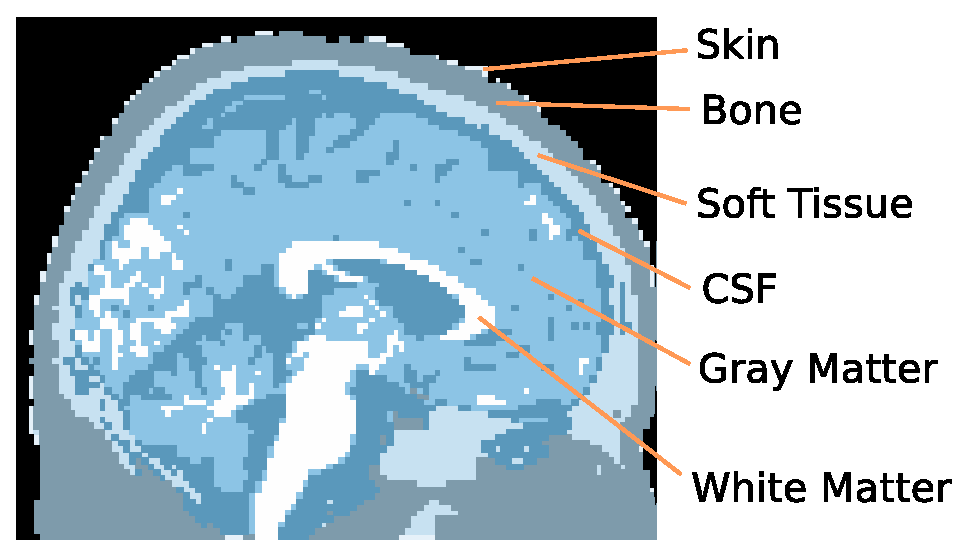
\includegraphics{segmented-head} 
    	\caption[Slice of the segmented head]{\label{fig:segmented} Slice of the segmented head. Each color represents a different tissue type.} 
    \end{figure}
    \begin{table*}[tb] 
    		\begin{tabular*}{\linewidth}{@{} l p{2.7cm}p{2cm}p{2.4cm}p{2.5cm}p{2cm}@{}}
    		  \toprule
    		  Tissue & $f_0$ \newline $100 \; ml/(g \; min)$ & $\rho$ \newline $kg/m^{3}$ & $c$ \newline $J \: kg^{-1} \: \degree C^{-1}$ & $k$ \newline $W \: m^{-1} \: \degree C^{-1}$ & $Q_{m}$ \newline $W/m^{3}$ \\
    		  \midrule
    			Bone & 3 & 1,080 & 2,110 & 0.65 & 26.1 \\
    			Cerebrospinal Fluid & 0 & 1,007 & 3,800 & 0.50 & 0 \\
    			Gray Matter & 67.1 & 1,035.5 & 3,680 & 0.565 & 15,575 \\
    			White Matter & 23.7 & 1,027.4 & 3,600 & 0.503 & 5,192 \\
    			Muscle & 3.8 & 1,041 & 3,720 & 0.4975 & 687 \\
    			Skin & 12 & 1,100 & 3,150 & 0.342 & 1,100 \\
    			\bottomrule
    		\end{tabular*}
    		\caption[Tissue-specific parameters]{\label{tbl:tissues} Tissue-specific parameters used to calculate the temperature change (values from~\citet{collins}).} 
    \end{table*}
  In order to begin the temperature calculating procedure, a model of the head must first be created.  Using SPM8 (\url{http://www.fil.ion.ucl.ac.uk/spm/}), we segmented a T1 contrast image of the head into five different tissue types: bone, cerebral spinal fluid, gray matter, white matter and soft tissue.  It was assumed that soft tissue voxels that are in contact with air are more appropriately labeled as skin, so in total we are left with a model of the head separated in to six tissue types (\cref{fig:segmented}).  The advantage this has is that we are able to use tissue specific parameters when doing the calculations, thereby improving the accuracy of the results.  The parameters used are available in~\cref{tbl:tissues}.  The code used to create the head matrix is discussed in~\cref{apdx:headmatrix}.

  
  % CALC EQUIL T
    % \FloatBarrier
    \subsection{\label{sec:calcequilT} Calculating the equilibrium temperature}
  The first step in calculating the temperature change is to know the resting state temperature for each voxel within the head. Our approach was to have the initial temperature for all tissue voxels set to 37\degree C and air voxels are kept at 24\degree C.  The starting temperature of the tissue does not affect the final resting state temperature; however, starting off at drastically different values could greatly increase the calculating time required before the temperature stabilizes. The finite difference implementation of Penne's Bioheat Equation (\cref{eq:3dbioheat}) is used to update the temperature (derivation provided in~\cref{sec:calcT}).  The temperature is updated until the temperature for every voxel has stabilized ($\frac{dT}{dt} < 10^{-6}$ \degree C/s).  Since temperature changes due to changes in neuronal activity are typically greater than $10^{-2}$ \degree C, a change in temperature less than $10^{-6}$ \degree C/s is sufficiently small that transient temperature changes are negligible and temperature can be considered stabilized.  The code used to calculate the equilibrium temperature is detailed in~\cref{apdx:findequil}.
  
  % CALC M AND F
    \subsection{\label{sec:calcmf} Calculating Metabolism and Blood Flow Changes from the BOLD response}
    %%%%  Table of values used in Sotero, 2011  %%%%%
    \begin{table*}[p]
      \caption[Parameters used in the single-voxel approximation]{\label{tbl:soteroparams} Parameters used to solve the single-voxel implementation of Penne's Bioheat Equation.  (modified from~\citet{sotero2011})}
        \begin{tabular*}{\linewidth}{lp{8.5cm}p{7cm}}
          \toprule
          Parameter & Meaning & Value \\
          \midrule
          T$_{a}$ & Arterial blood temperature & 37\degree C \\
          C$_{tissue}$ & Tissue Heat Capacity & 3.664 J/(gK) \\
          $\Delta H^{\circ}$ & Enthalpy released by oxidation of glucose & $4.7 10^{5}$ J \\
          $\Delta H_{b}$ & Enthalpy used to release O$_{2}$ from hemoglobin & $2.8 10^{4}$ J \\
          CMRO$_{2}\mid_{0}$ & Cerebral metabolic rate of O$_{2}$ consumption at rest & $0.0263 10^{-6}$ mol/(gs) \\
          CBF$\mid_{0}$ & Cerebral blood flow at rest & 0.0093 cm\textsuperscript{3}/(gs) \\
          $\rho_{b}$ & Blood density & 1.05 g/cm\textsuperscript{3} \\
          C$_{B}$ & Blood heat capacity & 3.894 J/(gK) \\
          $\tau$ & Time constant for conductive heat loss from the ROI to the surrounding tissue & 190.52 s \\
          a, b, c & Parameters of the gamma function fitted from E(f) vs. f & 0.4492, 0.2216, $-0.9872$ \\
          A & Maximum BOLD signal change & 0.22 \\
          $\alpha$ & Steady state flow-volume relation & 0.4 \\
          $\beta$ & Field-strength dependent parameter & 1.5 \\
          \midrule
          Variable & Meaning & \\
          \midrule
          m(t) & CMRO$_2$ normalized to baseline & \\
          f(t) & CBF normalized to baseline & \\
          T(t) & Temperature & \\
          W(t) & Lambert W Function & \\
          $\frac{\Delta S(t)}{S_0}$ & Change in BOLD signal normalized to rest & \\
          \bottomrule
        \end{tabular*}
    \end{table*}
    This is the critical step where we use fMRI BOLD data to calculate the normalized change in metabolism and blood flow.  The method used~\citep{sotero2011} is an assemblage of a couple other works~\citep{buxton2004,buxton1997,fox1988,leithner2009,lin2010,davis1998}. It starts by using the relation between metabolism and blood flow proposed by~\citet{buxton2004}:
    \begin{equation} \label{eq:mf}
      m(t)=f(t)\frac{E(t)}{E_0}
    \end{equation}
  where $E_0$ is the oxygen extraction at rest and $E(f)$ is
    \begin{equation} \label{eq:E}
      E(f)=1-(1-E_0)^{\frac{1}{f(t)}}
    \end{equation}
  in accordance with the oxygen limitation model~\citep{buxton1997}.  Combining~\cref{eq:mf} with~\cref{eq:E} yields
    \begin{equation} \label{eq:EmfCombined}
      m(t)=\frac{f(t)}{E_0}\left[1-(1-E_0)^{\frac{1}{f(t)}}\right]
    \end{equation}
  \Citet{sotero2011} goes about solving~\cref{eq:EmfCombined} by adjusting $E(t)$ data generated by~\cref{eq:E} and fitting it to the gamma function for the $f$ range (0.7--2.0) that is within experimentally reported values~\citep{fox1988,leithner2009,lin2010}:
    \begin{equation} \label{eq:gammafct}
      \frac{E(f)}{E_0}=af^{c}(t)e^{-bf(t)}
    \end{equation}
  where a, b and c are fitting parameters (values provided in~\cref{tbl:soteroparams}).  From this approximation we have the final form of metabolism:
    \begin{equation} \label{eq:m} 
      m(t)=af^{c+1}(t)e^{-bf(t)}.
    \end{equation}
  As proposed by~\citet{davis1998}, the BOLD signal changes ($\frac{\Delta S(t)}{S_0}$) can be described in terms of $m(t)$ and $f(t)$:
    \begin{equation} \label{eq:S}
      \frac{\Delta S(t)}{S_0} = \frac{S(t)-S_0}{S_0} = A(1-f^{\alpha-\beta}(t) m^\beta(t))
    \end{equation}
  Substituting~\cref{eq:m} into~\cref{eq:S} yields
    \begin{equation} \label{eq:mAndS}
      f(t)e^{-\frac{b \beta}{\alpha + \beta c}f(t)}=\left(\frac{\left(A-\frac{\Delta S(t)}{S_0}\right)}{A a^\beta}\right)^{\frac{1}{\alpha+\beta c}}
    \end{equation}
  where A is the maximum change in BOLD signal.  Multiplying each side by $-\frac{b\beta}{\alpha+\beta c}$ gives
    \begin{equation} \label{eq:mAndSmultiplied}
      -\frac{b\beta}{\alpha+\beta c} f(t)e^{-\frac{b \beta}{\alpha + \beta c}f(t)}=-\frac{b\beta}{\alpha+\beta c} \left(\frac{\left(A-\frac{\Delta S(t)}{S_0}\right)}{A a^\beta}\right)^{\frac{1}{\alpha+\beta c}}
    \end{equation}
  which can be solved by using the Lambert W function
    \begin{equation} \label{eq:lambertW}
      z=W(x)
    \end{equation}
  where $W(x)$ is a solution for z in the equation
    \begin{equation} \label{eq:lambertWsetup}
      z e^z = x
    \end{equation}
  Finally, $f(t)$ is obtained from~\cref{eq:mAndSmultiplied}
    \begin{equation} \label{eq:f}
      f(t)=\frac{\alpha+\beta c}{b \beta}W(y(t))
    \end{equation}
  where
    \begin{equation} \label{eq:y} 
    	y(t)=-\frac{b \beta}{\alpha+\beta c} \left[\frac{(A-\frac{S(t)}{S_{0}}-1)}{A a^{\beta}}\right]^{\left(\frac{1}{\alpha+\beta c}\right)} 
    \end{equation}
  is a function of the BOLD signal.  Using \cref{eq:m,eq:f,eq:y} allows for the metabolism and blood flow to be calculated from the BOLD signal (values used are provided in~\cref{tbl:soteroparams}).
  
    In order to process the files, the BOLD dataset is stored as a separate NIFTI (*.nii) file for each time step.  The first step in processing the data for temperature calculations is to determine a resting state BOLD signal ($S_0$).  The resting state is calculated by taking the voxel-wise mean of the data when the subject is at rest (i.e. the first and last 20 seconds).  This results in one data set where each voxel is a mean of all of the voxels at the location over time ($S_0$).  In order to calculate the metabolism and blood flow, the BOLD dataset needs to be normalized to this resting state ($\frac{\Delta S(t)}{S_0}$).  
    
    Once $\frac{\Delta S(t)}{S_0}$ is known for each time step, \cref{eq:m,eq:f,eq:y} can be used to calculate the metabolism and blood flow. The implementation of this procedure is discussed in~\cref{apdx:fmriprocessing}. 

  % CALC CHANGE IN T
    \subsection{\label{sec:calcT} Calculating the change in temperature in the active brain}
    As discussed in~\cref{sec:multivox}, the foundation of the model is Penne's Bioheat Equation,~\cref{eq:3dbioheat}.  The metabolism and blood flow time-courses calculated in~\cref{sec:calcmf} are used to scale the baseline heat production and blood profusion.  This, in turn, induces a change in the temperature.
    
    Penne's Bioheat Equation (\cref{eq:3dbioheat}) is implemented using the first-order forward finite difference method:
    \begin{equation}
      \label{eq:finitedifference}
      \dot{T}(t) \approx \frac{T(t+l)-T(t)}{l}
    \end{equation}
    where $T(t)$ is the temperature at time $t$ and $l$ is the time step size. Next, we can approximate $\nabla^{2} T$ by using the second order central finite difference method applied for each coordiante:
    \begin{align}
      \frac{\partial^2T(t;x,y,z)}{\partial x^2} &\approx \frac{T(t;x+h,y,z)-2 T(t;x,y,z)+T(t;x-h,y,z)}{h^2} \notag\\
      \frac{\partial^2T(t;x,y,z)}{\partial y^2} &\approx \frac{T(t;x,y+h,z)-2 T(t;x,y,z)+T(t;x,y-h,z)}{h^2} \notag\\
      \frac{\partial^2T(t;x,y,z)}{\partial z^2} &\approx \frac{T(t;x,y,z+h)-2 T(t;x,y,z)+T(t;x,y,z-h)}{h^2}\label{eq:fdspatial}
    \end{align}
where 
  \begin{equation}
    \label{eq:leplaceT}
    \nabla^{2} T = 
    \frac{\partial^2T(t;x,y,z)}{\partial x^2} + 
    \frac{\partial^2T(t;x,y,z)}{\partial y^2} + 
    \frac{\partial^2T(t;x,y,z)}{\partial z^2}
  \end{equation}
and the step size in each coordinate direction is given by $h$.  In the case of processing BOLD data, $h$ is the voxel size.
\Cref{eq:leplaceT} can be subtitued into Penne's Bioheat Equation~(\cref{eq:3dbioheat})
  \begin{equation}
    \rho c \dot{T} = k_x \frac{\partial^2 T}{\partial x^2} + k_y \frac{\partial^2 T}{\partial y^2} + k_z \frac{\partial^2 T}{\partial z^2} -\rho_{blood}f(t)wc_{blood}(T-T_{blood})+m(t)Q_{m} \label{eq:simplifiedbioheat}
  \end{equation}
  where $\dot{T}$ is the first-derivative of temperature with respect to time, $k_x$ is the thermal conductivity in the x-direction, $k_y$ is the thermal conductivity in the y-direction and $k_z$ is the thermal conductivity in the z-direction.
  Substituting~\cref{eq:fdspatial,eq:finitedifference} into~\cref{eq:simplifiedbioheat} yields
  \begin{align}
    \rho c \frac{T(t+l;x,y,z)-T(t;x,y,z)}{l} \approx \frac{1}{h^2} 
    & [k_x (T(t;x+h,y,z)-2 T(t;x,y,z)+T(t;x-h,y,z)) \notag\\
    & + k_y (T(t;x,y+h,z)-2 T(t;x,y,z)+T(t;x,y-h,z))\notag\\
    & + k_z (T(t;x,y,z+h)-2 T(t;x,y,z)+T(t;x,y,z-h))]\notag\\
    & -\rho_{blood}f(t)wc_{blood}(T-T_{blood})+m(t)Q_{m}
  \end{align}
  which is then rearranged to solve for $T(t+l;x,y,z)$
  \begin{align}
    \label{eq:fdfinal}
    T(t+l;x,y,z) \approx T(t;x,y,z) + \frac{l}{\rho c h^2} 
    & [k_x (T(t;x+h,y,z)-2 T(t;x,y,z)+T(t;x-h,y,z)) \notag\\
    & + k_y (T(t;x,y+h,z)-2 T(t;x,y,z)+T(t;x,y-h,z))\notag\\
    & + k_z (T(t;x,y,z+h)-2 T(t;x,y,z)+T(t;x,y,z-h))]\notag\\
    & -\rho_{blood}f(t)wc_{blood}(T-T_{blood})+m(t)Q_{m}
  \end{align}
  The time step size ($l$) can be picked arbitrarily, however the spatial step size ($h$) is limited to the voxel spacing.
  
  The final equation~(\cref{eq:fdfinal}) gives a method for calculating the next time step ($T(t+l)$) from the current time step ($T(t)$) for each voxel.  By using the central difference to solve $\nabla^2 T$, the voxels on all six sides of the current voxel are considered in the heat conduction.  The implementation of this equation is discussed in~\cref{apdx:tempCalcDynMF}.
  
% RESULTS
  \section{\label{sec:results} Results} 
   In order to understand the behavior of the model, we first applied it simulated BOLD data that was generated by convolving a boxcar function with the hemodynamic response function provided by SPM8.  After we understood the behavior of the model, we then applied it to experimental BOLD data that was collected by~\citet{dhamala}.

  %% THEORETICAL RESULTS %%
    \subsection{\label{sec:theoreticalresults} Using Synthetic BOLD Data}
    \FloatBarrier
    \begin{figure}[p] 
    	\begin{center}
    		\begin{tabularx}{\textwidth}{cc}
    			\raisebox{20px}{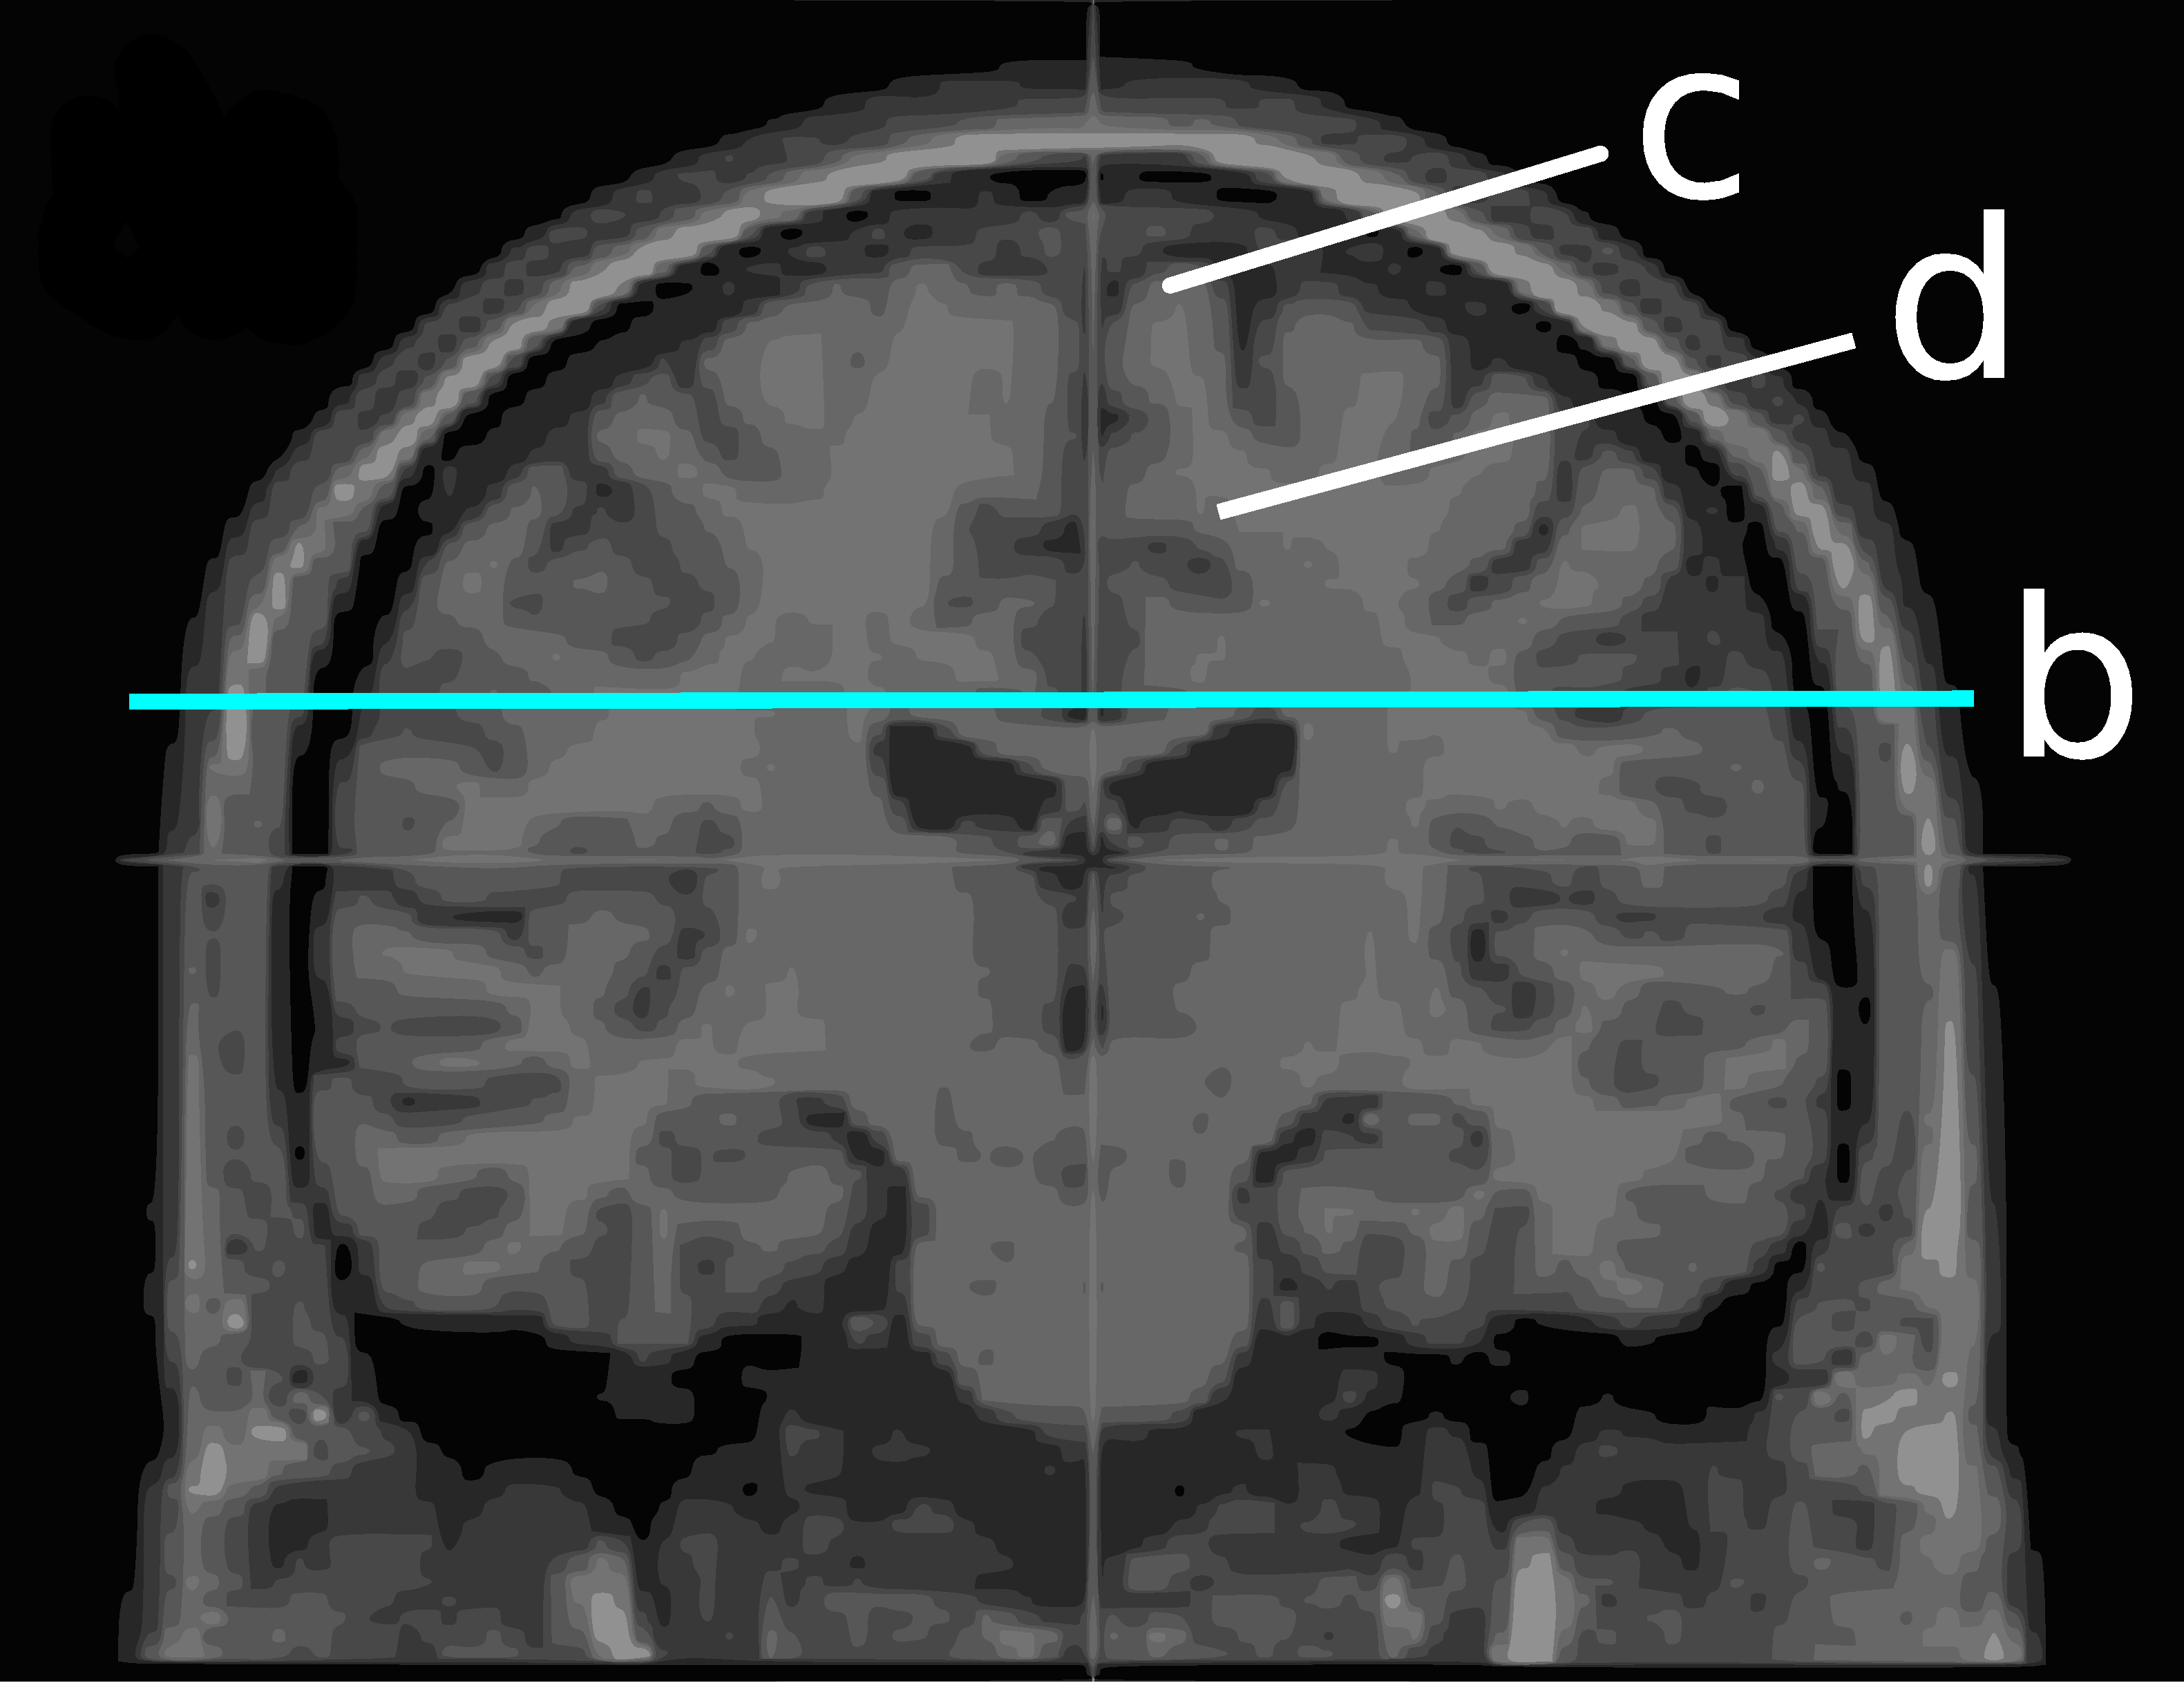
\includegraphics[width=0.36\textwidth]{headref}} & 
    			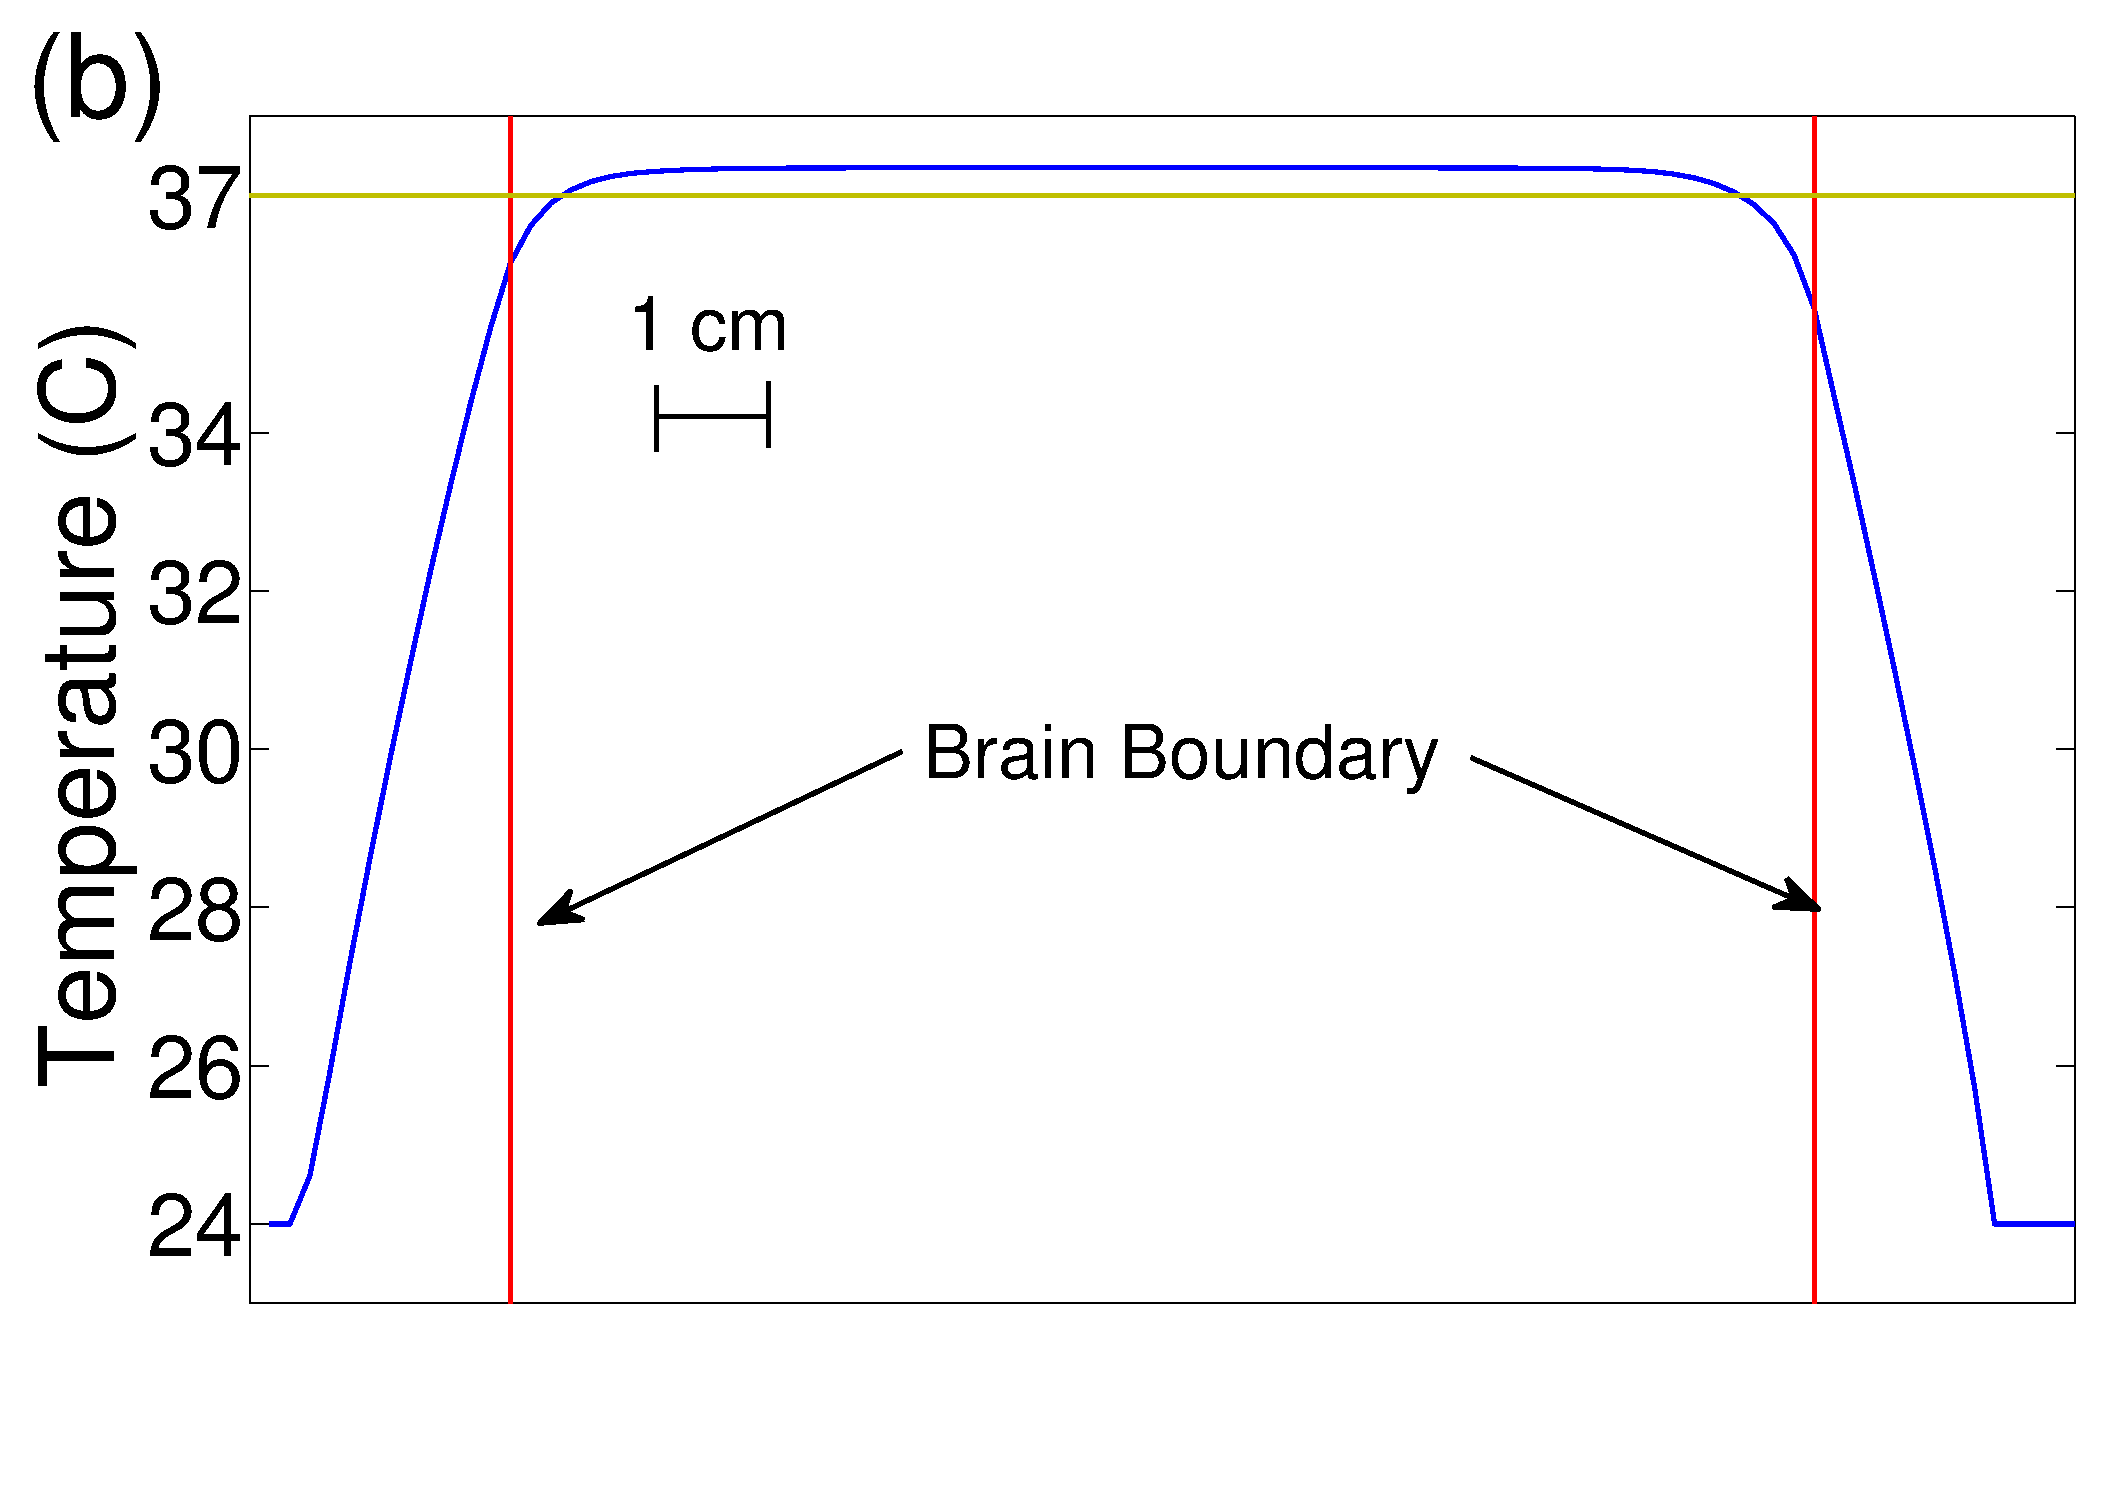
\includegraphics[width=0.5\textwidth]{equilibrium_temperature_0_55_52} \\
    			\multicolumn{2}{c}{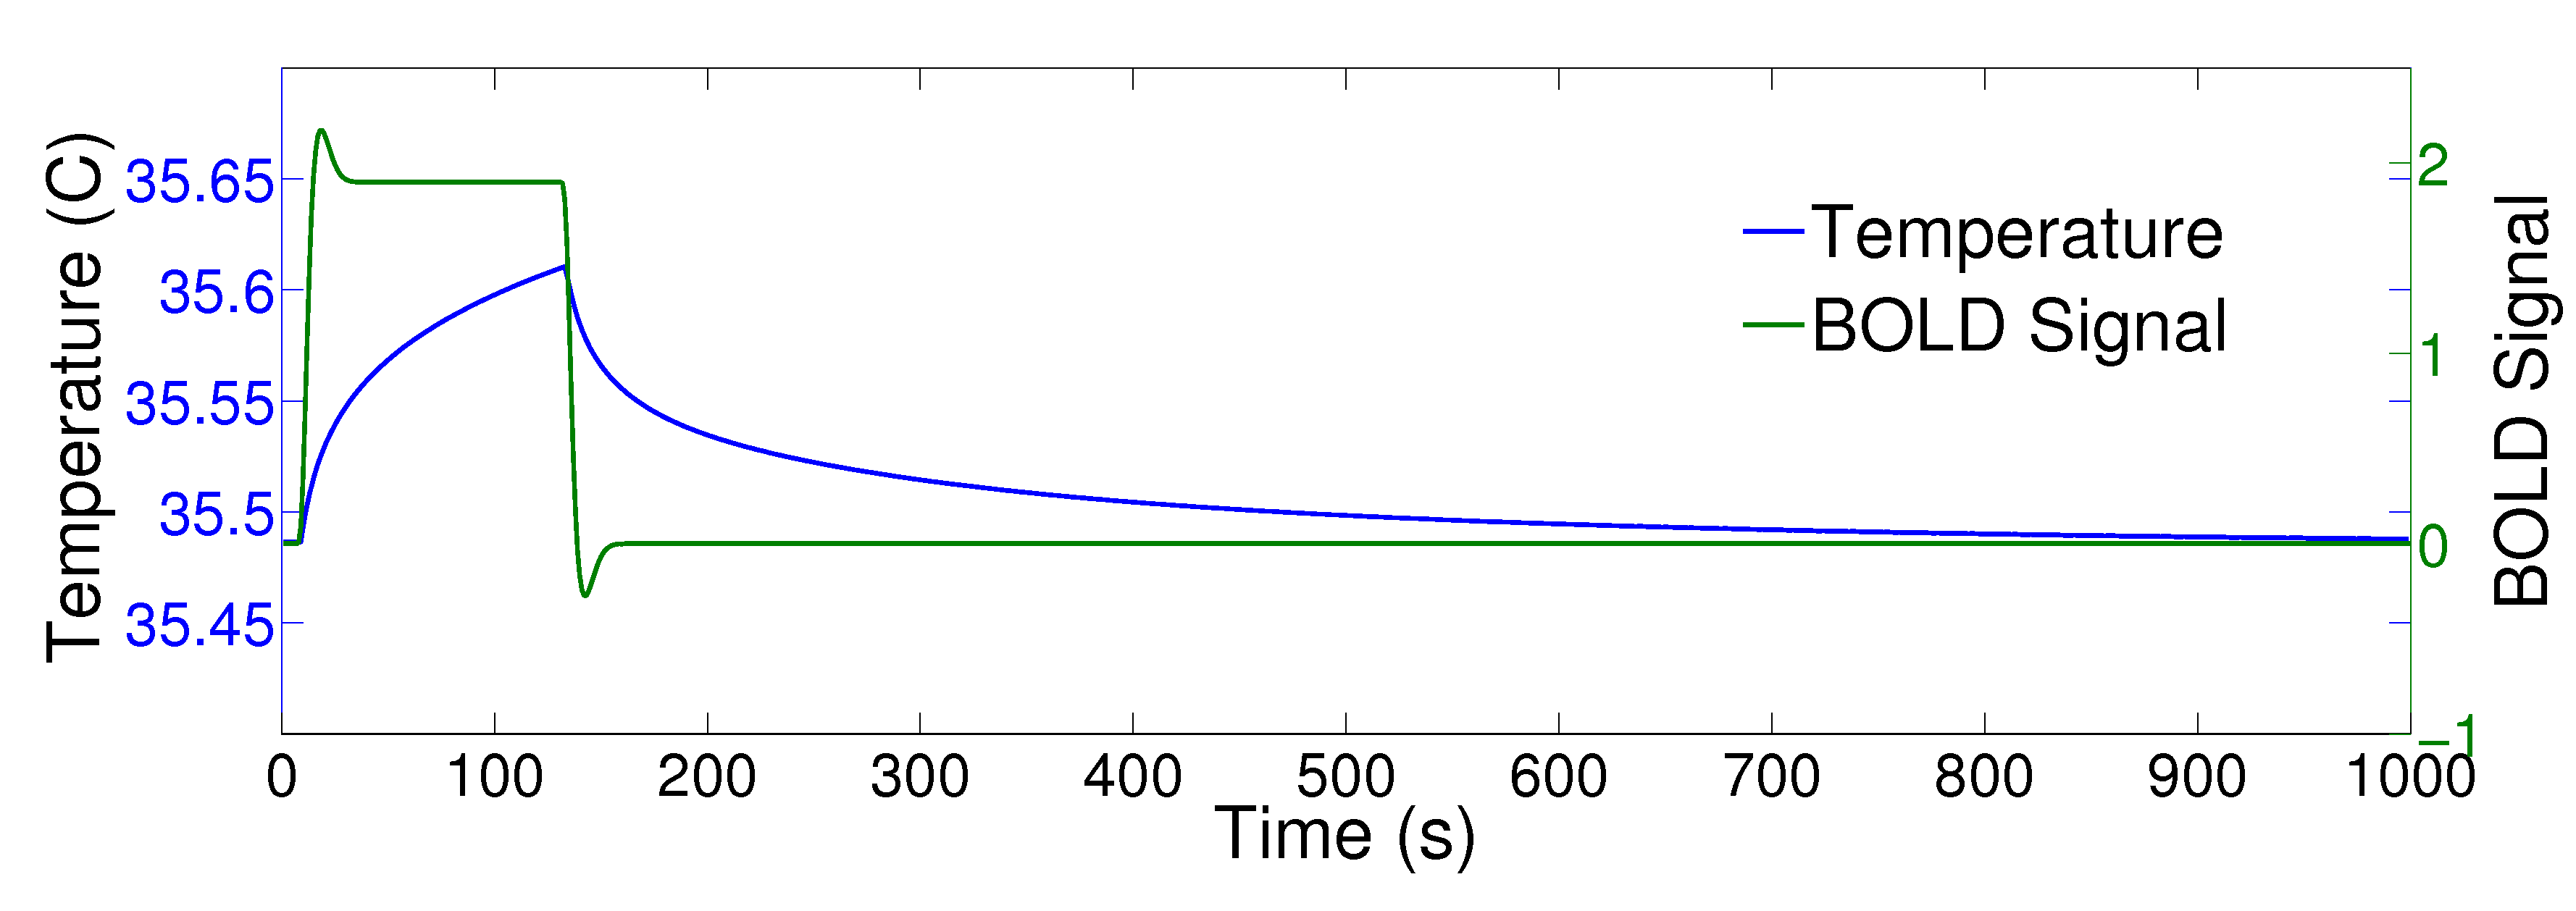
\includegraphics{sim_bold_(48_58_76)}} \\
    			\multicolumn{2}{c}{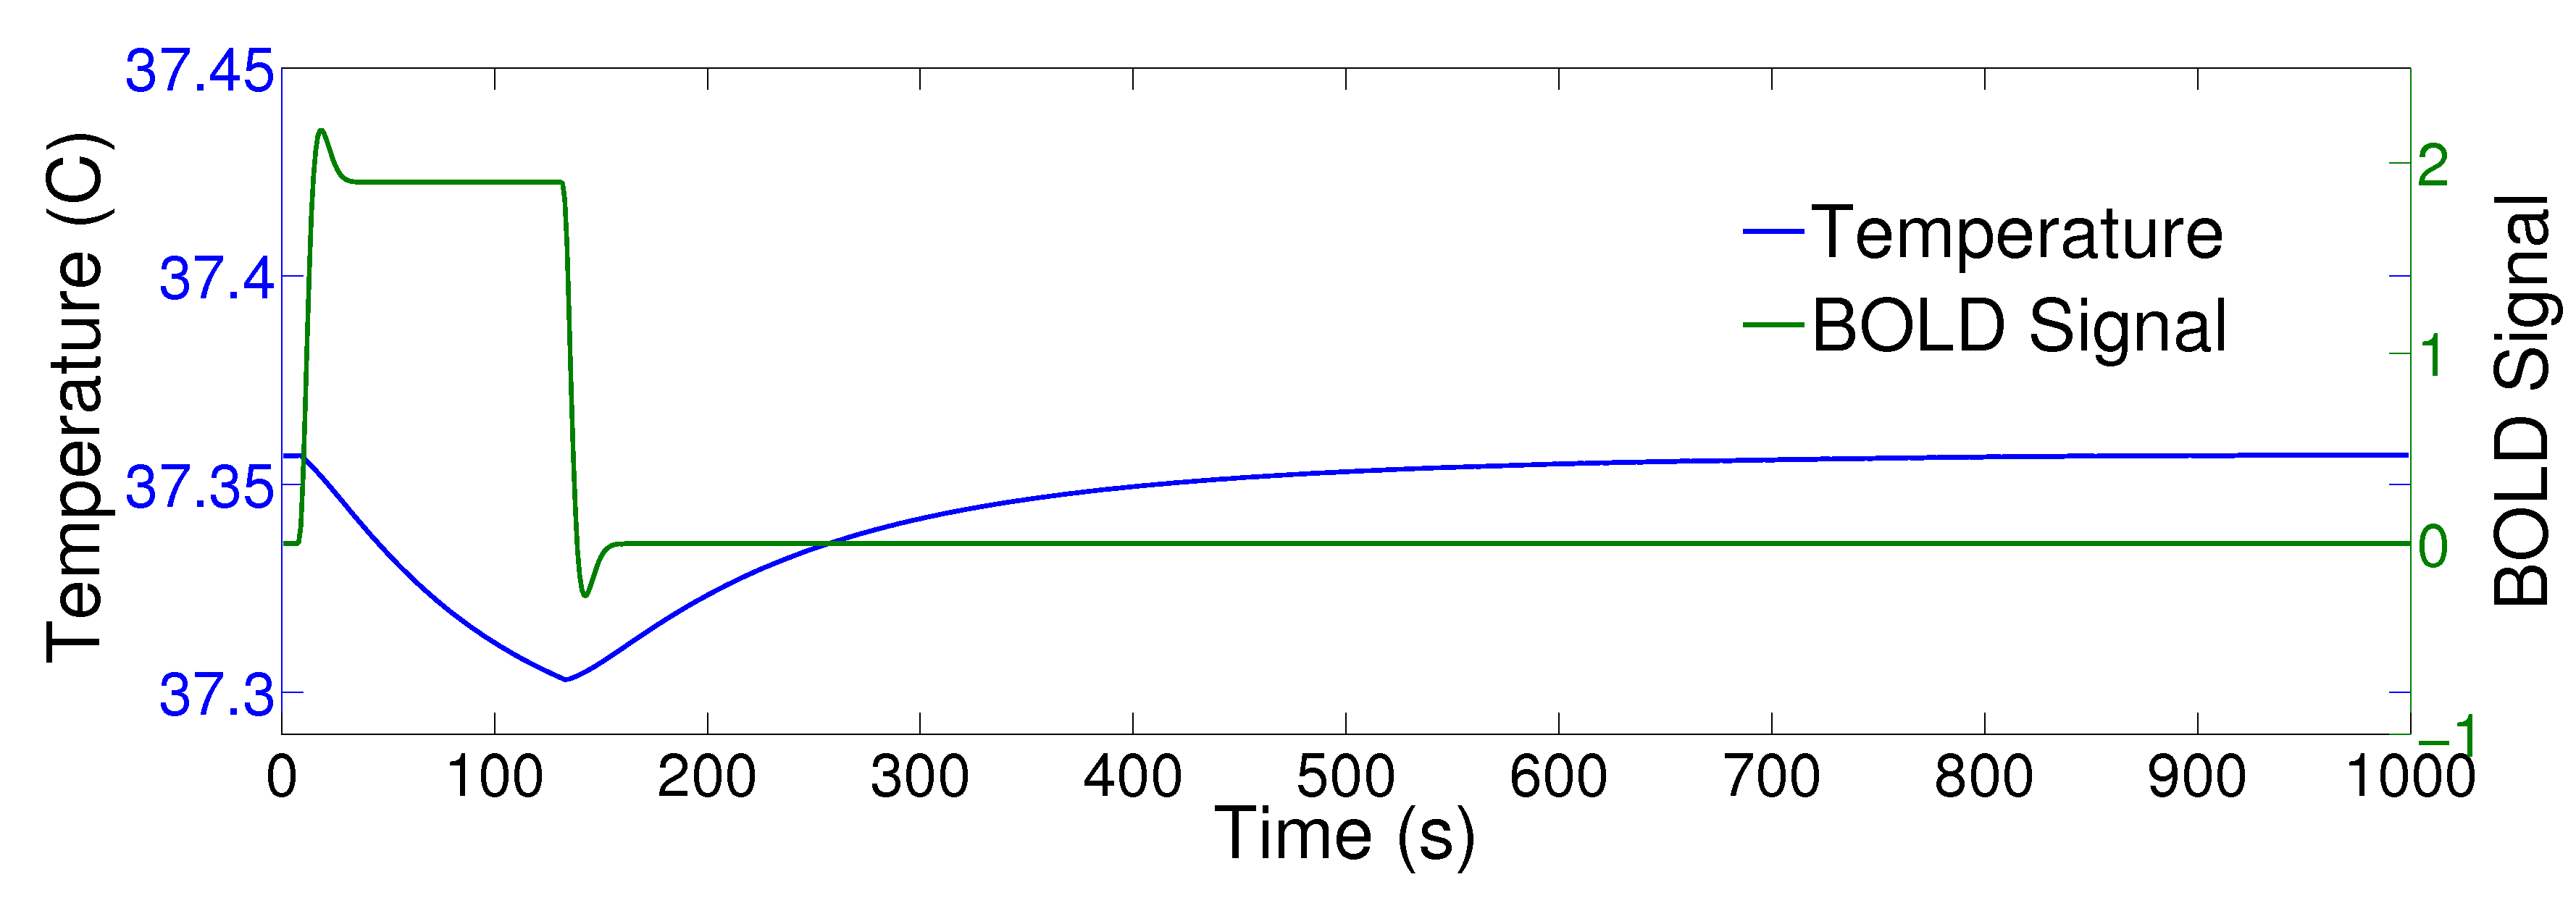
\includegraphics{sim_bold_(48_58_56)}}
    		\end{tabularx}
    	\end{center}
    	\caption[Temperature changes: simulated BOLD data]{\label{fig:simulateddata} Temperature changes using simulated BOLD signals. (a) Slice of the head (y = -12) with indicators of the locations for parts (b)-(d). (b) Equilibrium temperature along a line through the head. Red lines indicate the brain boundary and the gold line indicates the blood temperature (37\degree C) used for calculations. Inside the brain, a 4-6 mm thick shell is created where the equilibrium temperature is less than the blood temperature. Within this shell, (c) the temperature rises with increased brain activity while (d) tissue deeper in the brain experiences the opposite effect.} 
    \end{figure}
    To better understand the behavior of the tissue temperature model and the characteristics of temperature changes, BOLD activity was simulated in two ways: (i) from a nonlinear hemodynamic model \cite{friston2000} using stimulus or response function, or (ii) by convolving a boxcar function with the canonical hemodynamic response function provided by SPM 8 and corresponding temperature changes were calculated. Figure \ref{fig:simulateddata}(c,d) shows a typical simulated BOLD response used (green curve) along with the change in temperature (blue) for two voxels at different locations in the brain (locations indicated by Fig. \ref{fig:simulateddata}(a)). 
    
    Although both voxels have the same BOLD data, the demonstrate contrasting changes in temperature.  This can be best understood by considering the equilibrium temperature of each voxel.  Figure \ref{fig:simulateddata}(b) is a plot of the equilibrium temperature (blue line) along a line passing through the head (path indicated by the teal line in part (a) of the same figure). The vertical red lines indicate the boundary between the brain and surrounding tissues and the horizontal yellow line is an indication of the blood temperature (37\degree C). Two regions exist within the brain that lead to contrasting temperature behaviors.  
    
    The majority of the brain tissue is at a resting-state temperature that is less than the blood temperature (region 1).  For voxels within this region, a behavior like that shown in Fig.~\ref{fig:simulateddata}(d) is to be expected.  The primary contribution to an increase in the BOLD response is an increase in local blood flow.  Since the blood temperature is cooler than the tissue temperature, blood flow removes heat from the tissue thereby lowering the temperature.  Single-voxel models are able to account for this result because their assumptions about the location of a voxel are consistent with being located within this region.
    
    The second region is comprised of a thin (4--6 mm) layer of brain tissue that is closest to the surface of the head.  As a result of its proximity to the surface of the head, conductive heat lost to the air puts the resting-state temperature of voxels in this region below the arterial blood temperature.  As a result, when there is an increase in blood flow (increase in BOLD), the warmer blood will increase the voxel temperature (Fig.~\ref{fig:simulateddata}(c)).  Since single-voxel models approximate voxel conditions, they are unable to account for this region of tissue.
    
    Conduction is a slow process, so over shorter time scales (less than \Gtilde 10 minutes), conduction will contribute very little to the temperature change from a change in brain activity.  However, conduction plays an important role in determining the resting-state temperature.  
    
    The primary advantage with this model is that it accounts for the contribution of all of the voxels when determining the temperature, thus the direction of the temperature change depends on how far away from the surface of the head the voxel is. For voxels within a 4--6 mm shell near the surface of the brain, the temperature increases with increased activity (Fig. \ref{fig:simulateddata}(c)) while voxels deeper within the brain experience the opposite change (Fig. \ref{fig:simulateddata}(d)).
    
    %%  EXPERIMENTAl RESULTS %%
    \subsection{\label{sec:experimentalresults} Using Experimental BOLD Data}
    \FloatBarrier
    \begin{figure}[p] 
    	\begin{center}
    		$ 
    		\begin{array}{c}
    			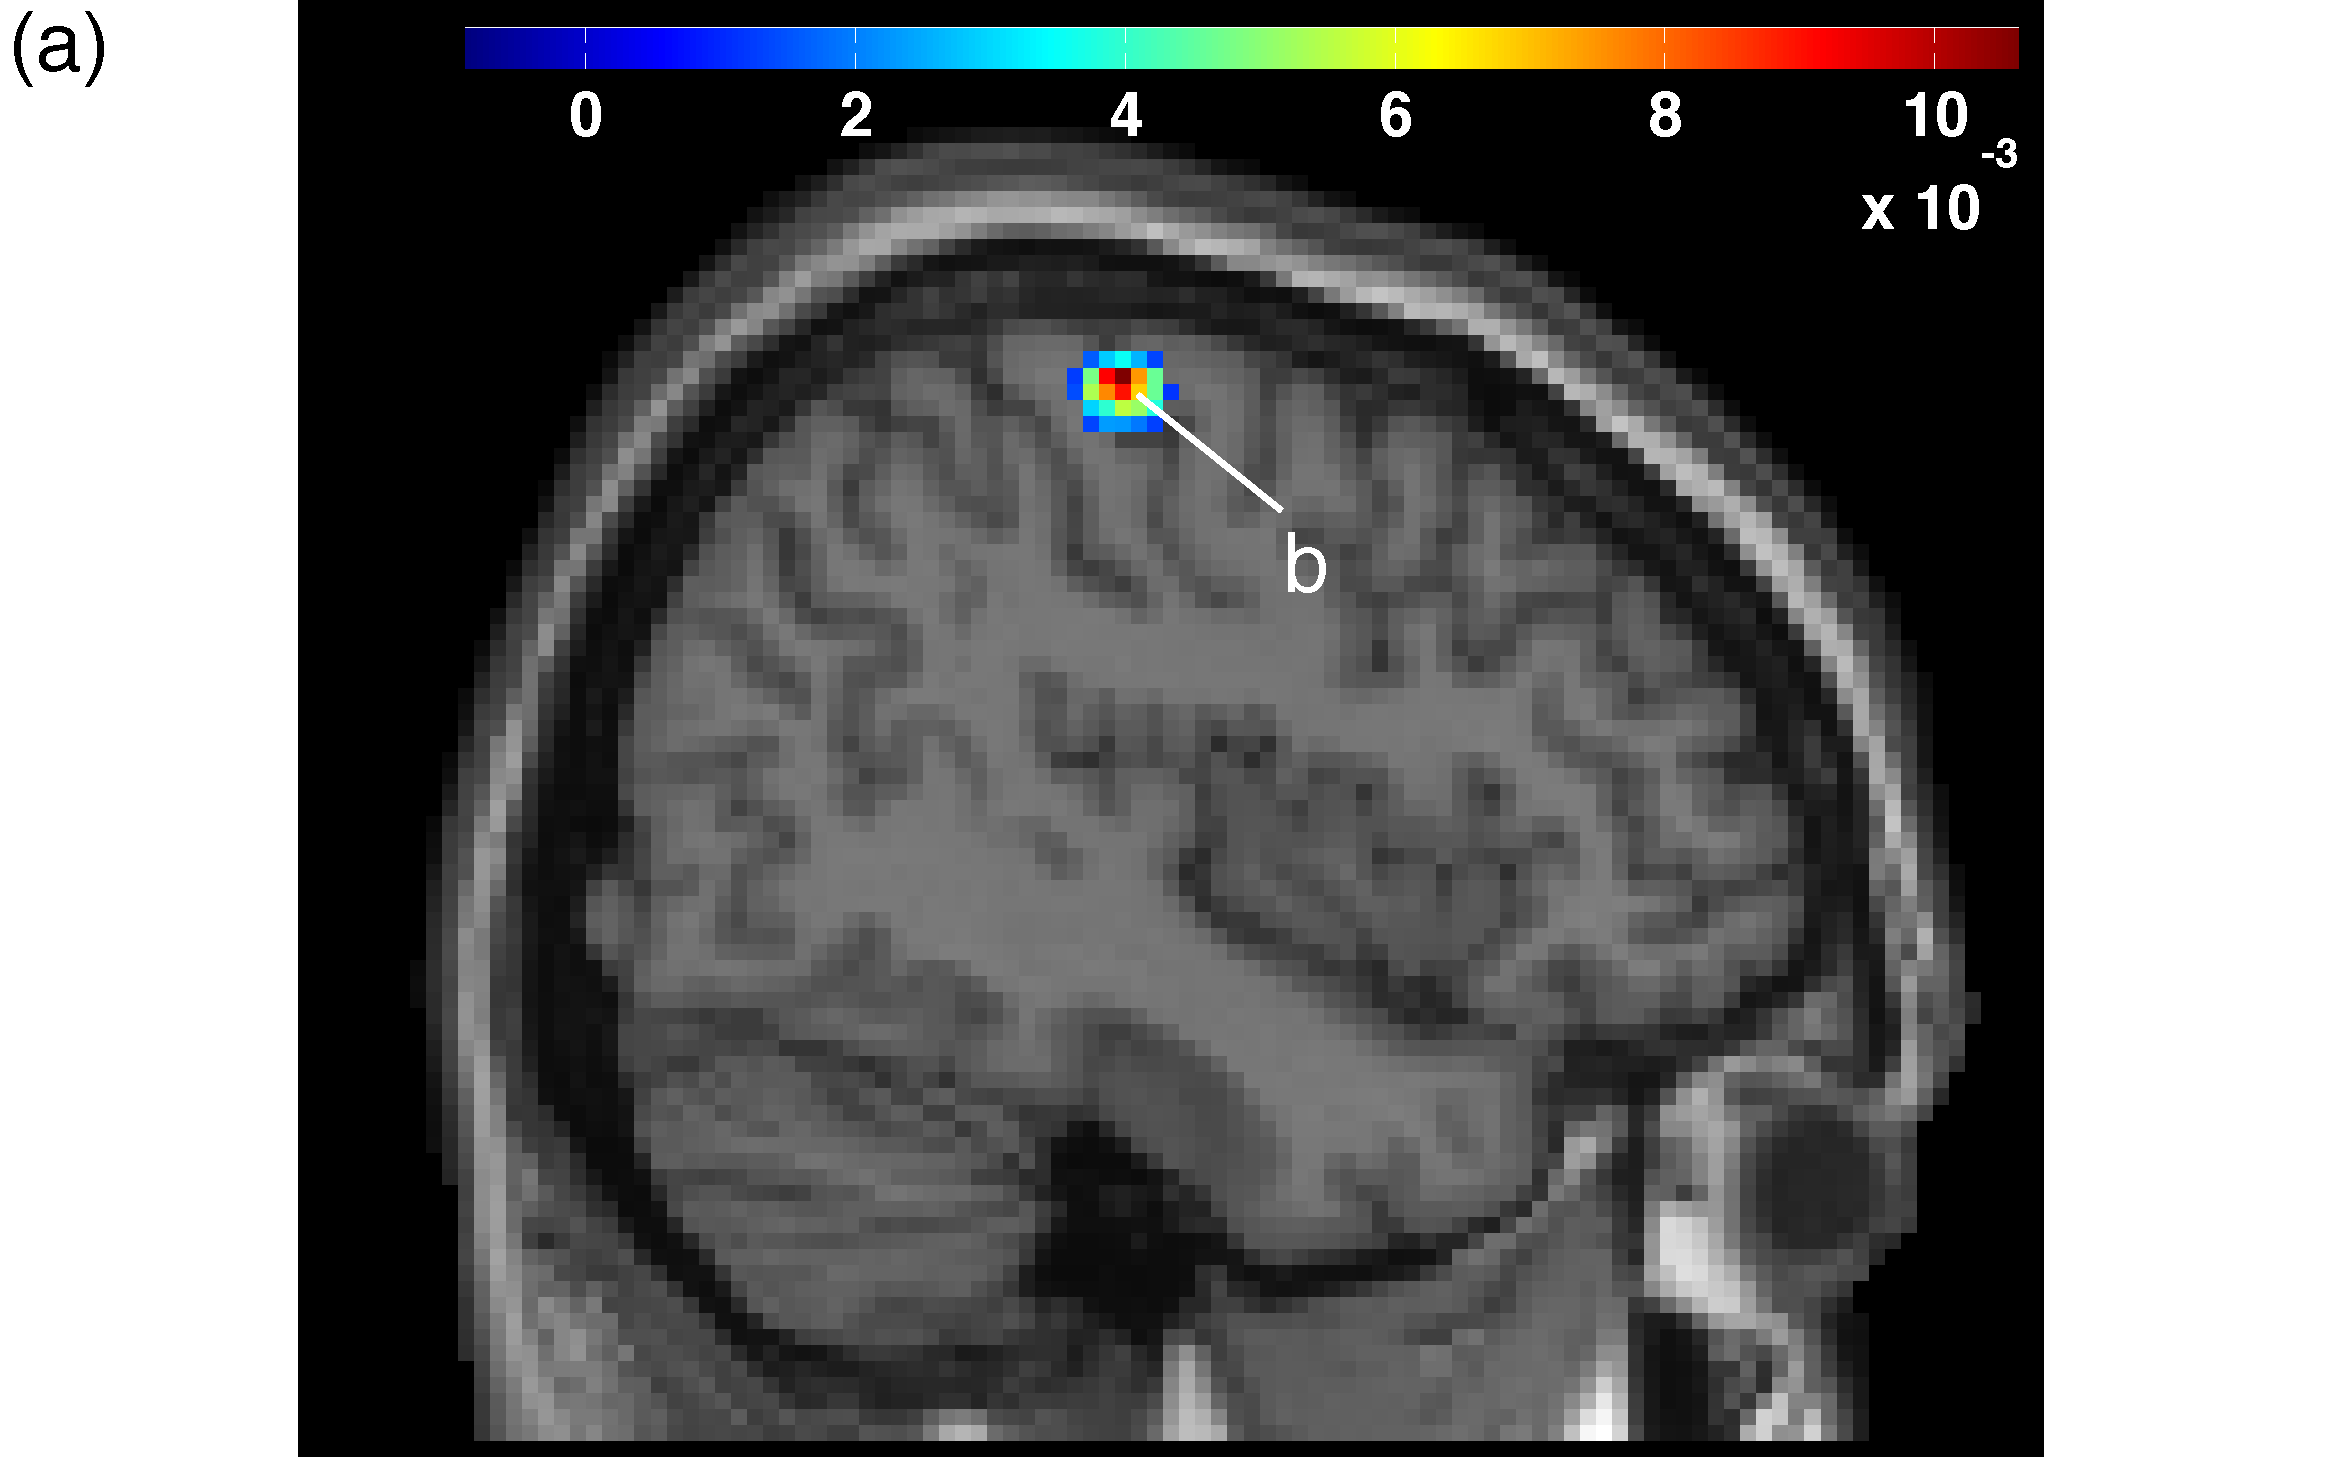
\includegraphics[width=0.9\linewidth]{slice_x_24} \\
    			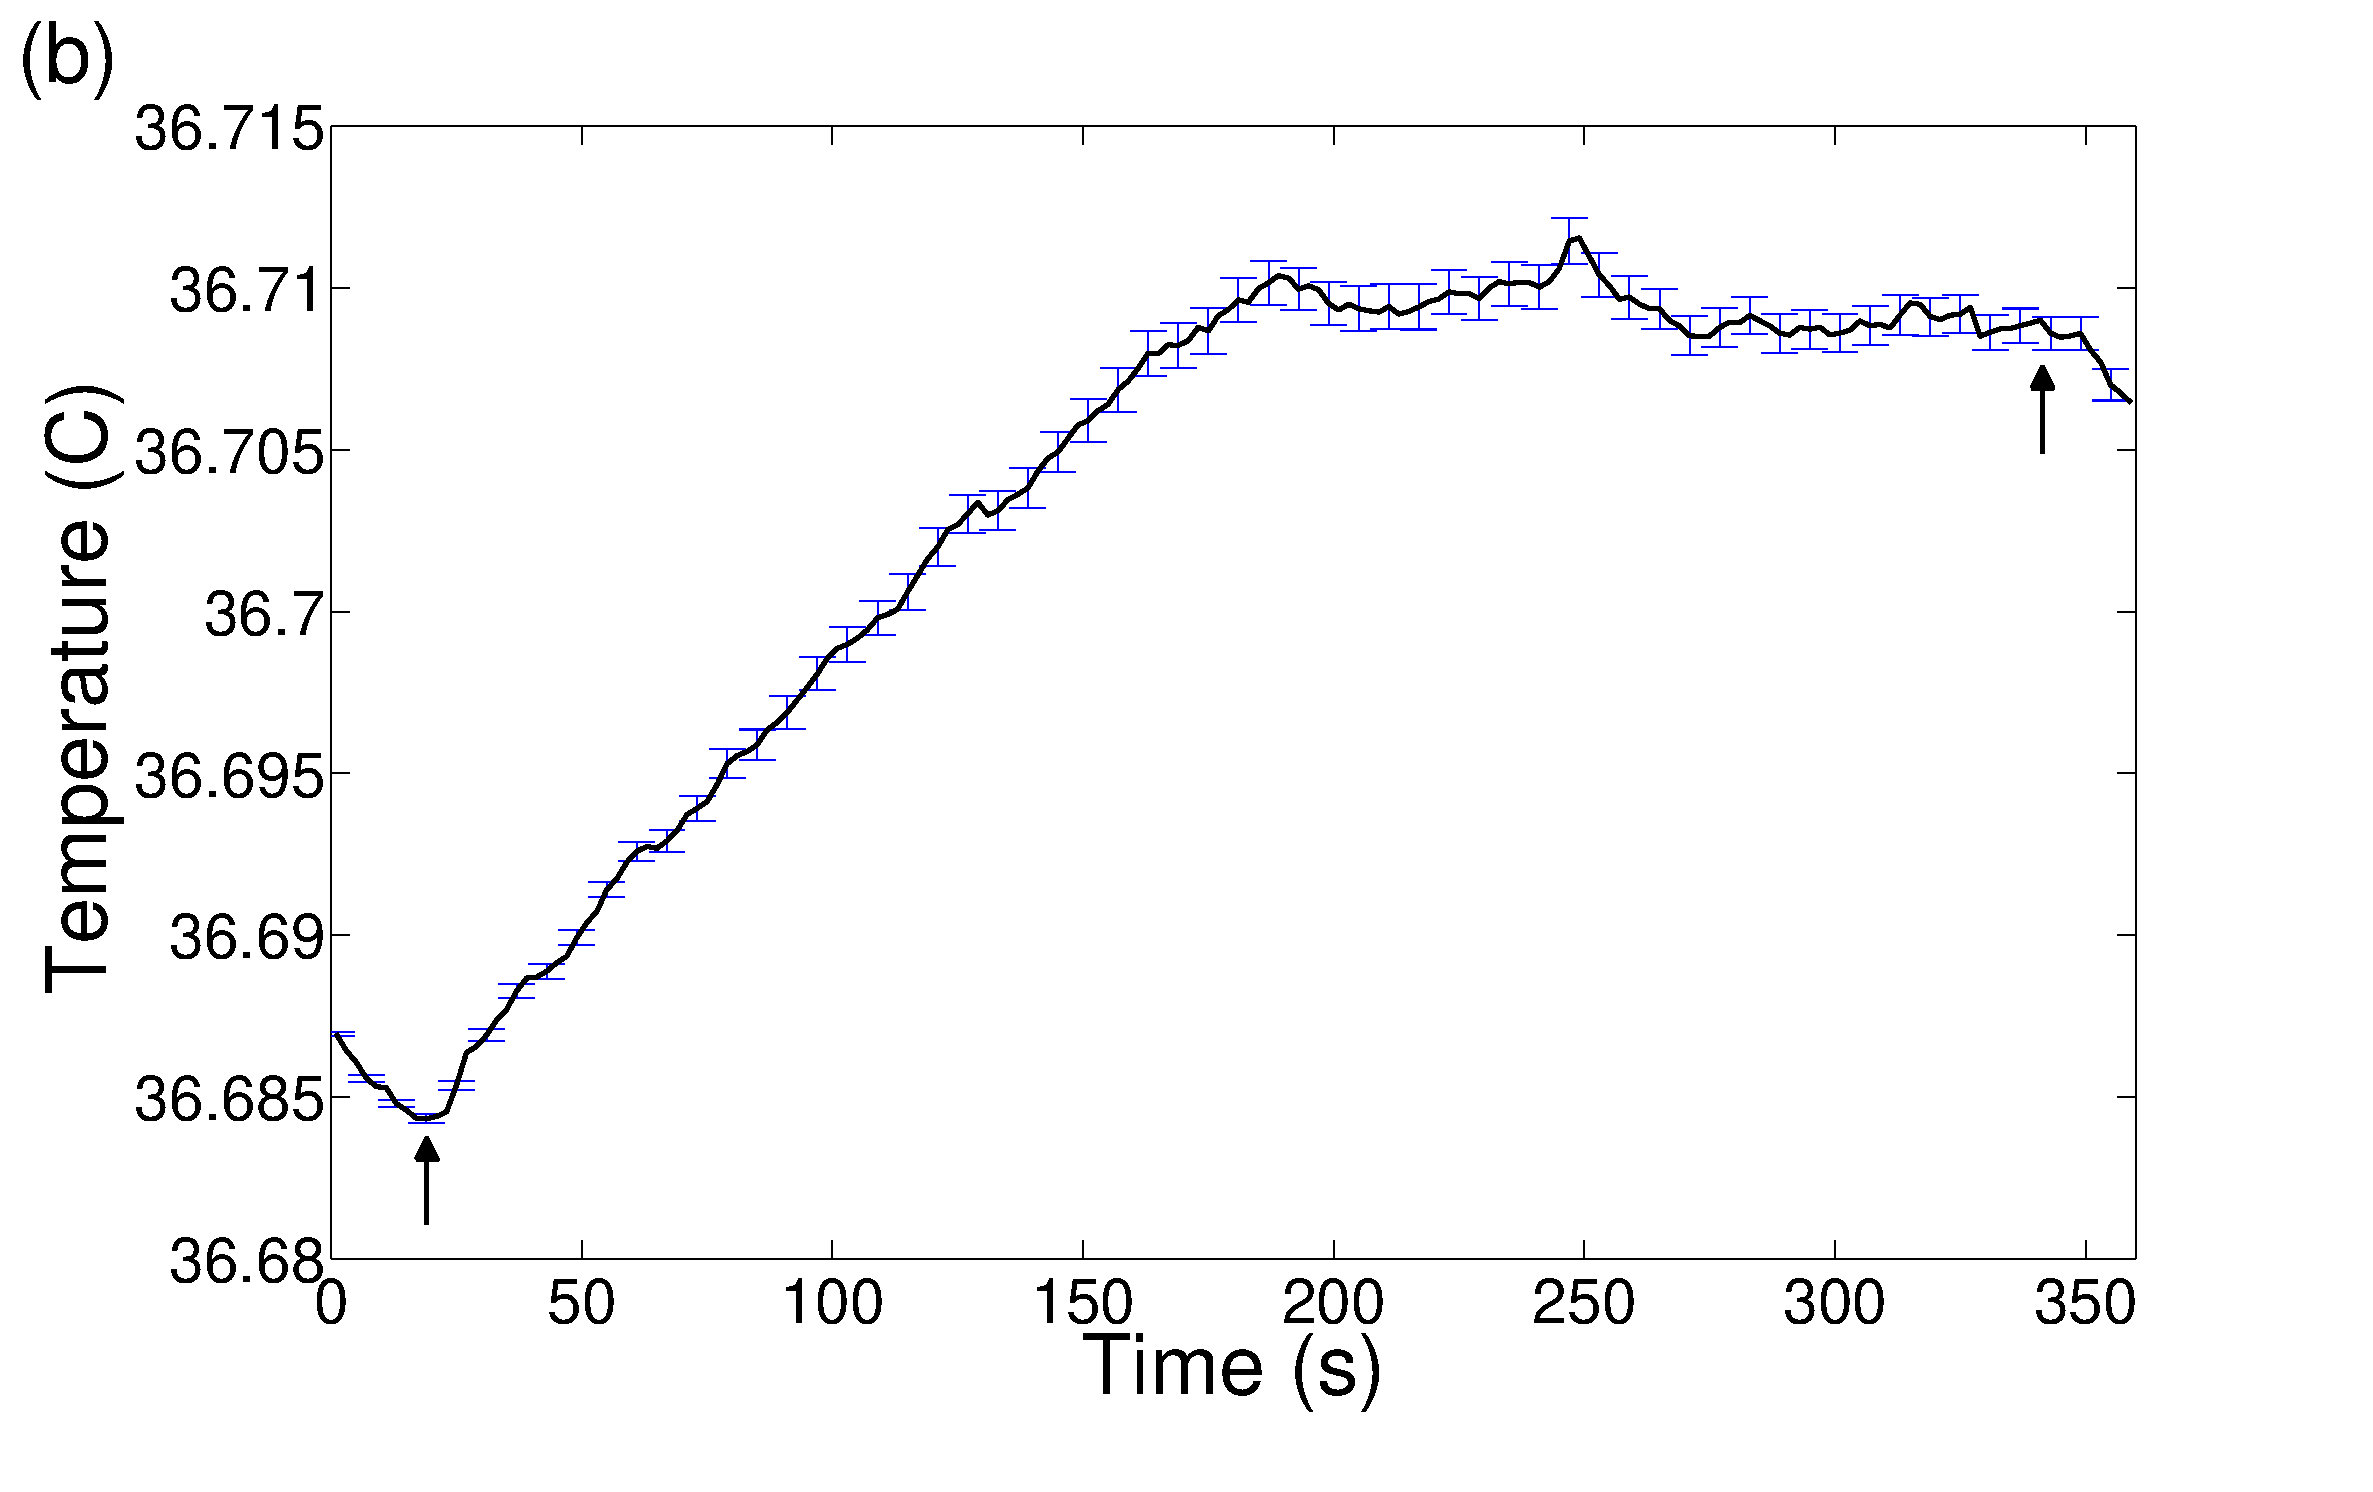
\includegraphics[width=0.9\linewidth]{avg_data_24_52_67} 
    		\end{array}
    		$ 
    	\end{center}
    	\caption[Temperature changes: experimental BOLD data]{\label{fig:realdata} Temperature calculated from a voxel within the motor cortex. (a) A slice (x = -44) showing the motor cortex warming during a finger-tapping task. (b) Temperature at a voxel within the motor cortex (-44, -24, 60) with standard error indicated by blue error bars (Arrows indicate task onset and conclusion, N=24).} 
    \end{figure}
    Data from a previous fMRI study~\citep{dhamala} was used to study the characteristics of temperature changes in a typical experiment. All participants in this experiment were right handed and between the ages of 23 and 27 years old.  Signed informed consent was collected from each one prior to participating in the study.  Institutional Review Boards of Emory University and Georgia State University approved this experiment. Twelve participants were asked to tap their right index fingers with rhythms of varying complexity for 320s. 
    
    This task resulted in a strong BOLD response in the motor cortex (\cref{fig:realdata}). The experiment included 20s of rest at the beginning and end of the tapping periods. Here, the resting state response level is calculated for each voxel by averaging across 40s of resting-state fMRI data. Using equations~\cref{eq:f,eq:m,eq:y}, the time-dependent change in blood flow and metabolism can be determined for each voxel. Finally, these values are used in conjunction with~\cref{eq:3dbioheat} to find the change in temperature throughout the brain. In this task, a temperature increase of approximately 0.02\degree C was observed in the motor cortex (\cref{fig:realdata}).  This value is well within the range of temperature changes observed in experimental measurements~\citep{mcelligott,kiyatkin,zeschke,george,tachibana}. 
    
    The increase rather than decrease in temperature in the motor cortex during a functional activity is consistent with the idea that the temperature of the blood in the capillaries is slightly greater than the baseline tissue temperature in superficial cortical regions; however, single-voxel models would predict the opposite effect.